\chapter{Background}
\label{ch.bkg}

% In this section, we introduce concepts central to the study of proton structure. The theoretical discussions will touch upon some concepts in quantum mechanics (e.g. probability amplitudes) special relativity (e.g. four-vectors), and particle physics (e.g. Feynman diagrams). Appendices \ref{app.quantum}, \ref{app.relativity}, and \ref{app.feynman} provide a quick review of such topics, intended for readers with some prior knowledge. For undergraduates interested in learning about the theory, below are a few textbook recommendation:
% \begin{itemize}
%     \item {\it Introduction to Quantum Mechanics} by Griffiths \& Schroeter \cite{Griffiths_Schroeter}
%     \item {\it Introduction to Elementary Particles} by Griffiths \cite{Griffiths}
%     \item {\it A Standard Model Workbook} by Moore \cite{Moore}
%     % \item {\it Quarks \& Leptons: An Introductory Course in Modern Particle Physics} by Halzen \& Martin \cite{Halzen_Martin}
% \end{itemize}

In this chapter, we introduce concepts central to the study of proton structure. We begin in Ch. \ref{sec.bkg_QCD} by describing the characteristics of quantum chromodynamics (QCD), the theory which describes the strong force responsible for nuclear phenomena. In Ch. \ref{sec.bkg_DIS}, we discuss the theoretical background of deep-inelastic scattering (DIS) experiments used to study proton structure. We then introduce the Electron-Ion Collider in Ch. \ref{sec.bkg_EIC}, its experimental goals, and the role flavor physics in Ch. \ref{sec.bkg_heavy_flavor}.

% Some of the theoretical discussions will touch upon some concepts in special relativity, such as four-vectors and Lorentz-invariance, although with minimal depth. For reference, we have defined and discussed the relevant concepts in Appendix \ref{sec.relativity}. 

(All formulas here will be expressed in natural units, with $\hbar=c=1$, which simplifies expressions for quantum and relativistic calculations. This choice sets the units of time and distance equal to each other, and also sets the units of mass, energy, momentum, equal to one another.)


%---------------------------------------------------------
\section{Quantum Chromodynamics (QCD)}
\label{sec.bkg_QCD}

%--------------------------
\subsection{The Standard Model and the strong force}

The Standard Model of particle physics is currently the best theoretical framework for understanding three of the four fundamental forces in nature: 
\begin{itemize}
    \item electromagnetism, responsible for the electric and magnetic phenomena we are most familiar with;
    \item the weak force, responsible for certain types of decays, such as the $\beta$-decay of radioactive nuclei; and
    \item the strong force, responsible for holding together atomic nuclei.
\end{itemize}
The backbone of the Standard Model is quantum field theory, which combines quantum mechanics and special relativity to accurately describe the interactions of highly energetic elementary particles. The last force, gravity, is described by the theory of general relativity and currently not able to be formulated in the language of quantum field theory.

%
\begin{figure}[h!]
    \centering
    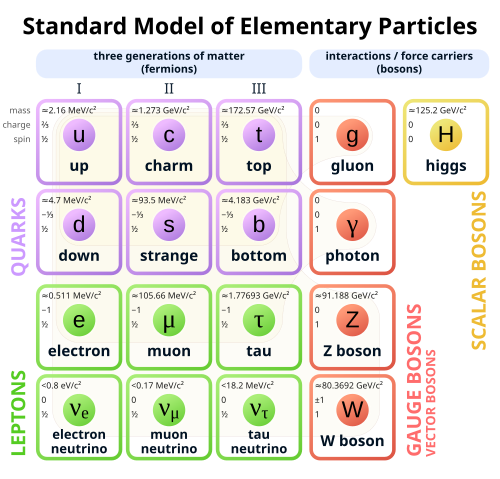
\includegraphics[width=0.6\linewidth]{gallery/background/standard_model.png}
    \caption{Particles of the Standard Model. Figure from \cite{sm}.}
    \label{f.sm}
\end{figure}
%
The particles in the Standard model are tabulated in Fig. \ref{f.sm}. The fermions are the particles which compose all visible matter, and the bosons are the ones which mediate the three fundamental forces between the particles. Nuclear physics is mainly concerned with the strong force, formulated through the theory of quantum chromodynamics (QCD), which describes the interactions between quarks and gluons. The particles which participate in strong-force interactions carry a property known as {\it color charge}, which is analogous to the electric charge in electromagnetism but comes in three values: ``red", ``blue", and ``green". Unlike the photons which mediate the electromagnetic force, the gluons which mediate the strong force also carry color charge themselves. Thus, gluons interact with each other, leading to highly complex and nonlinear dynamics.

%--------------------------
\subsection{The strong coupling constant}

For each force in the Standard Model, there is a characteristic {\it coupling} ``constant" which describes the strength of the associated interactions. For electromagnetism, the coupling is the fine structure constant $\alpha\approx 1/137$, which is a very small number and remains relatively constant across energy scales. In contrast, the strong coupling $\alpha_S$ is large at the low energies of our everyday experience and decreases as energy increases. This leads to the phenomena of {\it color confinement} at low energies and  {\it asymptotic freedom}. Color confinement describes the phenomenon in which the QCD interactions are so strong that at low energies, quarks are always found in color-neutral bound states called {\it hadrons}. Bound states of three quarks, such as protons and neutrons, are known as baryons, and bound states of two quarks (one quark and one antiquark) are known as mesons. On the opposite end of the energy spectrum, {\it asymptotic freedom} describes the phenomenon in which $\alpha_S$ becomes weak enough at high energies to allow quarks and gluons to exist as nearly free particles. This results in the production of quark-gluon plasma, a hot and dense ``soup" of free quarks and gluons, in extremely high energy collisions.

Due to the peculiar behavior of $\alpha_S$, studying the behavior of quarks and gluons within hadrons is challenging. It is impossible to resolve individual quarks and gluons at low energies, and in high energy collisions, we tend to break apart the hadrons we wish to study. Thus, there is still much we do not know about how quarks and gluons are distributed inside of hadrons, and how the hadron properties, such as mass and spin, arise from the interactions of the internal quarks and gluons. In the next section, Ch. \ref{sec.bkg_DIS}, we discuss the process of deep-inelastic scattering, the most common method for studying the structure of protons (and other hadrons).

%---------------------------------------------------------
\section{Imaging the proton through deep-inelastic scattering (DIS)}
\label{sec.bkg_DIS}

We can probe the structure of the proton by scattering an electron beam off a proton target and measuring what happens to the scattered electrons. In general scattering experiments, many measurements relate to an observable known as the cross section $\sigma$, which describes the probability of interaction between the scattering particles. In this section, we introduce the concept of cross sections in high energy experiments, and we discuss how such measurements for deep-inelastic electron-proton scattering can reveal information about proton structure.

%-----------------------------
\subsection{Cross sections in particle physics}
\label{sec.bkg_cross_section}
%
\begin{figure}[h!]
    \centering
    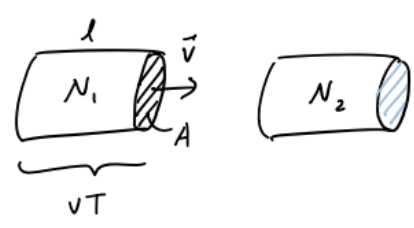
\includegraphics[width=0.5\linewidth]{gallery/background/cross_section.png}
    \caption{Scattering of two particle beams.}
    \label{f.cross_section}
\end{figure}
%
To illustrate the role of cross sections in particle physics, we follow the discussions in Ch. 14 of {\it A Standard Model Workbook} by Thomas Moore \cite{moore}. Imagine taking a snapshot of two particle beams traveling toward each other, as in Fig. \ref{f.cross_section}. In this snapshot of time interval $T$, beam 1 contains $N_1$ particles, beam 2 contains $N_2$, and their relative velocity is $\mathbf{v}$. Each beam can be approximated by a cylinder of volume $V$ and cross-sectional area $A$. The scattering cross section $\sigma$ relates the flux of incoming particles to the rate of scattering $\Gamma$ per volume,
\begin{equation}
    {\rm flux} \cdot \sigma = \frac{\Gamma}{V} \ .
    \label{eqn.sigma_beam}
\end{equation}

Let us consider the lab frame, in which the particles in beam 2 are at rest and the particles in beam 1 are traveling at $\mathbf{v}$. Here, the length of beam 1 is $|\mathbf{v}|T$. The total incoming flux is
\begin{equation}
    {\rm flux} = \frac{N_1|\mathbf{v}|}{V}\frac{N_2}{V} = \frac{N_1N_2}{AVT} \ ,
    \label{eqn.flux}
\end{equation}
where $N_1|\mathbf{v}|/V = N_1/AT$ is the flux of particles in beam 1, and $N_2/V$ is the density of particles in beam 2. The rate of scattering is
\begin{equation}
    \Gamma = \frac{{\rm Prob}_{1,2\rightarrow1',2'}}{T}N_1N_2,
    \label{eqn.rate}
\end{equation}
where ${\rm Prob}_{1,2\rightarrow1',2'}$ is the probability that a particle from beam 1 and a particle from beam 2 scatter into particles 1' and 2'. Since we are dealing with quantum particles, this probability is given by the squared amplitude for the initial state (particles 1 and 2) transitioning into the final state (particles 1' and 2') via time evolution. Thus, $\Gamma$ is better known as the {\it transition rate}. Additionally, in relativistic high energy collisions, the final state particles may not be the same species as the initial particles. (For example, an electron and positron can annihilate and produce a quark-antiquark pair.)

Substituting Eq. \eqref{eqn.flux} and \ref{eqn.rate} into \ref{eqn.sigma_beam},
\begin{equation}
    \left(\frac{N_1N_2}{VT}\right) \frac{\sigma}{A} = {\rm Prob}_{1,2\rightarrow1',2'}\left(\frac{N_1N_2}{VT}\right) \ .
\end{equation}
Thus, the cross section
\begin{equation}
    \sigma = A \cdot {\rm Prob}_{1,2\rightarrow1',2'}
\end{equation}
represents the effective area of interaction and is directly proportional to the probability of scattering between two particles. 
% For further discussion on this interpretation, Griffiths Ch. 6 \cite{Griffiths} draws a more detailed analogy between $\sigma$ and the Classical cross section through a geometric description of scattering. 

In high energy experiments, we can measure the cross section in terms of {\it luminosity} $\mathcal{L}=N_1N_2/AT$, where
\begin{equation}
    \sigma = \frac{\Gamma}{\mathcal{L}} \ .
\end{equation}
In scattering calculations, we generally work with the slightly more abstract differential cross section
\begin{equation}
    d\sigma = \frac{|\mathcal{M}|^2}{{\rm flux}} d{\rm Lips} \ ,
\end{equation}
where $\mathcal{M}$, called the {\it invariant amplitude}, represents the probability amplitude for the scattering process, and the {\it Lorentz-invariant phase space} $d{\rm Lips}$ represents the density of possible final states. $d{\rm Lips}$ is commonly written in terms of angular coordinates $d\Omega$, energy $dE$, momenta $d^3\mathbf{p}$, or other physical quantities. We say that the cross section is ``differential" in energy, momenta, etc. to indicate that it is measured as a function of such quantities.

% For $2\rightarrow 2$ interactions in which 2 initial particles of four-momenta $p_1$ and $p_2$ scatter into 2 final particles with four-momenta $p_1'$ and $p_2'$, we have a formula known as {\it Fermi's Golden Rule}:
% \begin{equation}
%     d\sigma = S \frac{(2\pi)^4\delta^{(4)}(p_1+p_2-p_1'-p_2') |\mathcal{M}|^2}{4\sqrt{(p_1 \cdot p_2)^2-m_1^2m_2^2}}\frac{d^3\mathbf{p}_1'}{(2\pi)^32E_1'}\frac{d^3\mathbf{p}_2'}{(2\pi)^32E_2'} \ ,
%     \label{eqn.golden_rule}
% \end{equation}

% where
% \begin{equation}
% \begin{aligned}
%     {\rm flux} &= \frac{2E_1|\mathbf{v}|}{V}\frac{2E_2}{V} = \frac{4\sqrt{(p_1 \cdot p_2)^2-m_1^2m_2^2}}{V^2} \\
%     \dot{P} &=\frac{(2\pi)^4\delta^{(4)}(p_1+p_2-p_1'-p_2') |\mathcal{M}|^2}{V^4}  \\
%     dN' &= \frac{Vd^3\mathbf{p}_1'}{(2\pi)^32E_1'}\frac{Vd^3\mathbf{p}_2'}{(2\pi)^32E_2'} \ ,
%     \label{eqn.cross_section_pieces}
% \end{aligned}
% \end{equation}

% where $\mathbf{p}_i$ is the spatial three-momentum of particle $i$ and $m_i^2=p_i^2=E_i^2-|\mathbf{p}_i|^2$ is the mass squared of particle $i$.

% Instead of delving into the derivation of Eq. \eqref{eqn.golden_rule} (which can be found in particle physics textbooks such as Griffiths Ch. 6 \cite{Griffiths} and Moore Ch. 14 \cite{Moore}),
% % and Halzen \& Martin Ch. 4 \cite{Halzen_Martin}), 
% here we provide a qualitative explanation of the important pieces. The most interesting quantity is the invariant amplitude $\mathcal{M}$. This piece contains the process-dependent parts of ${\rm Prob}_{1,2\rightarrow 1',2'}$, thus capturing all the physics of the interaction. The $\delta$-function encodes conservation of four-momentum, requiring that the initial four-momentum $p_1+p_2$ minus the final four-momentum $p_1'+p_2'$ is zero. The factors $d^3\mathbf{p}_i'/(2\pi)^32E'_i$ represent the density of momentum states for each final state particle.
% % All the factors of $2E_i/V$ result from the conventional normalization of incoming and outgoing wavefunctions, which gives $N_i=2E_i$ particles in the total interaction volume $V$. 
% Finally, the factor $S=1/n!$ out front is a degeneracy factor to prevent double-counting, where $n$ is the number of indistinguishable final state particles.
% % (For example, if the final state consists of two electrons, then $S=1/2$.)
% In Ch. \ref{sec.bkg_ep}, we will discuss the cross section for $ep$ scattering processes and how they can capture information about proton structure.

% Imagine taking a snapshot of two particle beams traveling toward each other, as in Fig. \ref{f.cross_section}. In this snapshot of time interval $T$, beam 1 contains $N_1$ particles, beam 2 contains $N_2$, and their relative velocity is $\mathbf{v}$. Each beam can be approximated by a cylinder of volume $V$ and cross-sectional area $A$. The scattering cross section $\sigma$ relates the total number of incoming particles to the number of scattered particles (i.e. the particles that actually interacted),
% \begin{equation}
%     N_{\rm incoming} \cdot \sigma = N_{\rm scattered} \ .
%     \label{eqn.cross_section}
% \end{equation}

% Let us consider the lab frame, in which the particles in beam 2 are at rest and the particles in beam 1 are traveling at $\mathbf{v}$. Here, the length of beam 1 is $|\mathbf{v}|T$. Normalized by the volume and time interval of the interaction, the number of incoming particles is given by
% \begin{equation}
%     \frac{N_{\rm incoming}}{VT} = \frac{N_1|\mathbf{v}|}{V}\frac{N_2}{V} = \frac{N_1N_2}{AVT} \ ,
%     \label{eqn.incoming}
% \end{equation}
% where $N_1|\mathbf{v}|/V = N_1/AT$ is the flux of particles in beam 1, and $N_2/V$ is the density of particles in beam 2. The number of scattering particles is given by
% \begin{equation}
%     \frac{N_{\rm scattered}}{VT} = \dot{P}N_1N_2 = \frac{|S_{fi}|^2}{VT}N_1N_2 \ ,
%     \label{eqn.scattered}
% \end{equation}
% where $\dot{P}=|S_{fi}|^2/VT$ is the scattering probability per volume per time. $S_{fi}$, called the S-matrix element, is the amplitude for the initial states transitioning into the final states through time evolution. As with any quantum process, squaring this amplitude, $|S_{fi}|^2$, gives us the transition probability.

% Substituting equations \ref{eqn.incoming} and \ref{eqn.scattered} into Eq. \eqref{eqn.cross_section},
% \begin{equation}
%     \left(\frac{N_1N_2}{VT}\right) \frac{\sigma}{A} = |S_{fi}|^2\left(\frac{N_1N_2}{VT}\right) \ .
% \end{equation}
% Thus, the cross section $\sigma = A \cdot |S_{fi}|^2$ represents the effective area of interaction and is directly proportional to the scattering probability. In high energy experiments, we measure the cross section in terms of beam luminosity $\mathcal{L}=N_1N_2/AT$ and the total interaction rate $\Gamma_{\rm tot}=N_1N_2\cdot|S_{fi}|^2/T$ \ ,
% \begin{equation}
%     \sigma = \frac{\Gamma_{\rm tot}}{\mathcal{L}} \ .
% \end{equation}

% Generally, we work with the slightly more abstract differential cross section
% \begin{equation}
%     d\sigma = \frac{\dot{P}}{f} dN' \ ,
% \end{equation}
% where $dN'$ is the density of final states and is proportional to angular coordinates $d\Omega$, energy $dE$, or other quantities we can measure. For any $2\rightarrow 2$ interaction in which 2 initial particles of four-momenta $p_1$ and $p_2$ scatter into 2 final particles with four-momenta $p_1'$ and $p_2'$,
% \begin{equation}
%     d\sigma = \frac{1}{n!}\frac{(2\pi)^4\delta^{(4)}(p_1+p_2-p_1'-p_2') |\mathcal{M}|^2}{4\sqrt{(p_1 \cdot p_2)^2-m_1^2m_2^2}}\frac{d^3\mathbf{p}_1'}{(2\pi)^32E_1'}\frac{d^3\mathbf{p}_2'}{(2\pi)^32E_2'} \ ,
%     \label{eqn.diff_cross_section}
% \end{equation}
% where
% \begin{equation}
% \begin{aligned}
%     \dot{P} &= \frac{|S_{fi}|^2}{VT}=(2\pi)^4\delta^{(4)}(p_1+p_2-p_1'-p_2') |\mathcal{M}|^2  \\
%     f &= 2E_1|\mathbf{v}|2E_2 = 4\sqrt{(p_1 \cdot p_2)^2-m_1^2m_2^2} \\
%     \rho &= \frac{d^3\mathbf{p}_1'}{(2\pi)^32E_1'}\frac{d^3\mathbf{p}_2'}{(2\pi)^32E_2'} \ ,
%     \label{eqn.cross_section_pieces}
% \end{aligned}
% \end{equation}
% with $\mathbf{p}_i$ being the spatial three-momentum of particle $i$ and $m_i^2=p_i^2=E_i^2-|\mathbf{p}_i|^2$ being the mass squared of particle $i$. The most interesting quantity in Eq. \eqref{eqn.diff_cross_section} is $\mathcal{M}$, called the invariant amplitude, which is essentially the non-trivial part of $S_{fi}$ and contains all the physics of the interaction. The $1/n!$ out front is a degeneracy factor to prevent double-counting, where $n$ is the number of indistinguishable final state particles. (For the $ep$ scattering processes we will consider, all final state particles will be distinguishable, so $1/n!=1$.) The $\delta$-function piece encodes conservation of four-momentum, requiring that the initial four-momentum $p_1+p_2$ minus the final four-momentum $p_1'+p_2'$ is zero. We will not delve further into the derivations for the expressions in Eq. \eqref{eqn.cross_section_pieces}, but these can be found in particle physics textbooks such as Griffiths Ch. 6 \cite{Griffiths} and Aitchison \& Hey Ch. 6 \cite{Aitchison_Hey}. In the next subsection \ref{sec.bkg_ep}, we will discuss the invariant amplitude $\mathcal{M}$ for various $ep$ scattering processes.

%-----------------------------
\subsection{Elastic $e\mu$ scattering: a first look at Feynman diagrams}
\label{sec.bkg_feynman}
Before delving into the details $ep$ scattering, let us first introduce {\it Feynman diagrams}, an essential tool for calculating cross sections in particle physics, and the common kinematic variables (Ch. \ref{sec.bkg_emu}). As an example, we will consider a simpler but related process: elastic electron-muon scattering $e^-\mu^-\rightarrow e^-\mu^-$.

%
\begin{figure}[h!]
    \centering
    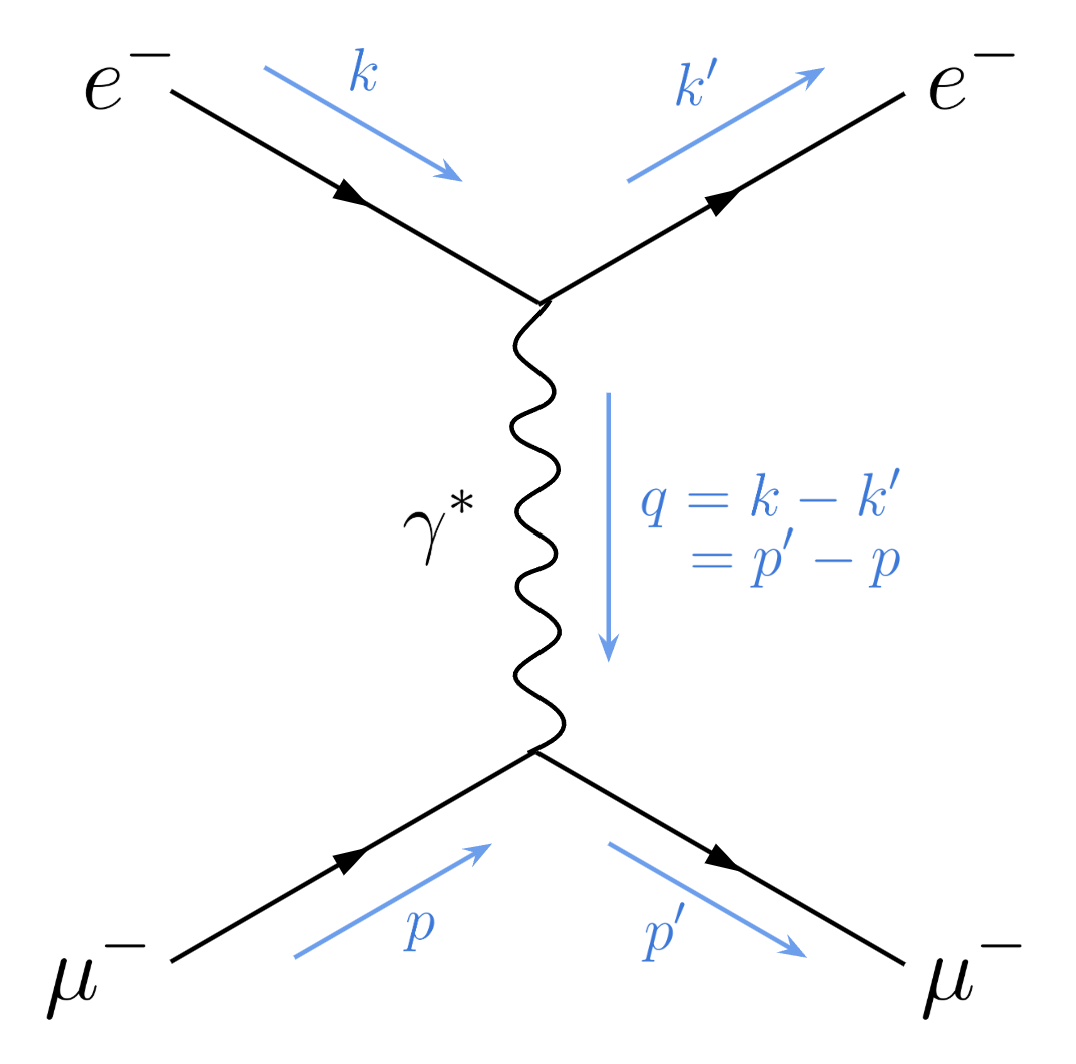
\includegraphics[width=0.4\linewidth]{gallery/background/emu_emu.png}
    \caption{Leading order Feynman diagram for elastic electron-muon scattering, $e^-(k) + \mu^-(p) \rightarrow e^-(k') + \mu^-(p')$. Four-momenta are labeled in blue.}
    \label{f.emu_emu}
\end{figure}
%
The Feynman diagram for the $e\mu$ scattering is shown in Fig. \ref{f.emu_emu}. We read the diagram from left to right, with the initial state particles on the left and final state particles on the right. Conventionally, fermions like electrons and muons are drawn as 
\begin{tikzpicture}
\begin{feynman}
\diagram {
  a -- [fermion] b
};
\end{feynman}
\end{tikzpicture} \ ,
and photons are drawn as 
\begin{tikzpicture}
\begin{feynman}
\diagram {
  a -- [photon] b
};
\end{feynman}
\end{tikzpicture} \ .
These particle lines are called {\it propagators}. The blue arrows in Fig. \ref{f.emu_emu} denote the four-momentum of each particle. (A four-momentum is an object that combines the energy $E$ and three-dimensional momentum vector $\mathbf{p}$ into a single vector, $p\equiv(E,\mathbf{p})=(E,p_x,p_y,p_z)$. For more background on four-momenta and four-vectors, see Appendix \ref{sec.relativity}). 

Altogether, the diagram depicts an electron with four-momentum $k$ and a muon with four-momentum $p$ traveling toward each other, exchanging a photon with four-momentum $q$, then scattering off with new four-momenta $k'$ and $p'$. We can see that this is an electrodynamic interaction, since it is mediated by the exchange of a photon.

To clarify, Feynman diagrams do not illustrate what the interaction physically looks like in space, so we should avoid interpreting the particles as interacting at some location or at some particular time. Instead, the diagrams serve as mathematical tools for calculating cross sections. From quantum field theory, there are a set of {\it Feynman rules} that associate a specific factor with every vertex and propagator, which multiply together to produce an expression for the invariant amplitude $\mathcal{M}$.

%
\begin{figure}[h!]
    \centering
    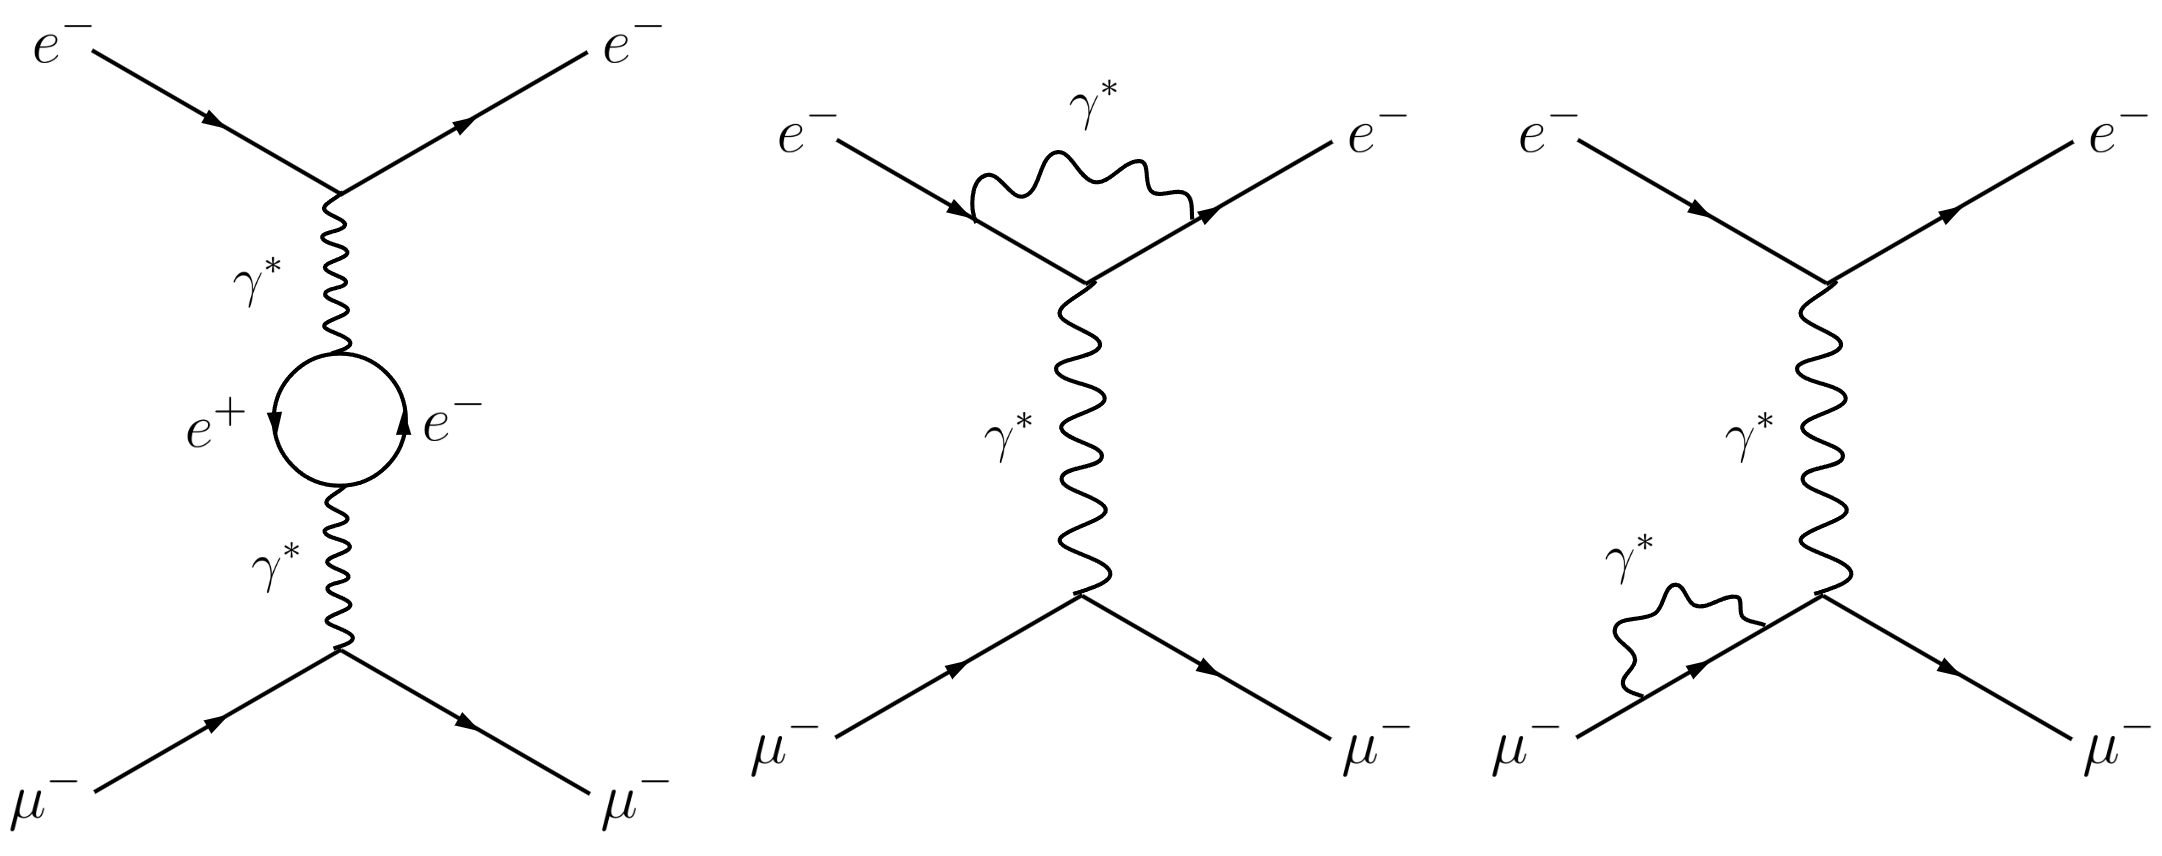
\includegraphics[width=0.8\linewidth]{gallery/background/emu_nlo.png}
    \caption{Examples of next-to-leading order Feynman diagrams for $e^-\mu^-\rightarrow e^-\mu^-$.}
    \label{f.emu_nlo}
\end{figure}
%
Actually, Fig. \ref{f.emu_emu} is the first term in an infinite series of Feynman diagrams for $e
\mu$ scattering, and the true invariant amplitude $\mathcal{M}$ is the sum of all their contributions. We refer to Fig. \ref{f.emu_emu} as the {\it leading order} diagram, which means that it contains the lowest number of vertices (two in this case) needed for the interaction to occur. All other diagrams are of higher order, containing more vertices. Fig. \ref{f.emu_nlo} shows a few examples of Feynman diagrams for $e\mu$ scattering at next-to-leading order, which all involve four vertices.

The Feynman rules tell us that every vertex comes with a factor proportional to the {\it electromagnetic coupling}, $\alpha=e^2/4\pi\approx1/137$, which determines the interaction strength in electrodynamic processes. Summing all the possible diagrams, we have
\begin{equation}
    \mathcal{M} = \mathcal{M}^{(1)}(\alpha^2) + \mathcal{M}^{(2)}(\alpha^4) + \mathcal{M}^{(3)}(\alpha^8) + \cdots \ ,
\end{equation}
where $\mathcal{M}^{(i)}$ is the $i$-th term in a {\it perturbative} expansion in powers of $\alpha^2$. Since the value of $\alpha$ is very small ($\alpha^2\approx5.3\times10^{-5}\ll1$), higher-order terms become progressively smaller ($\mathcal{M}^{(i+1)}\ll \mathcal{M}^{(i)}$), so they act like incremental corrections (or perturbations) to the previous terms. For electrodynamic processes like $e\mu$ scattering, the leading order term alone is enough to give a reasonable approximation of $\mathcal{M}$.

%-----------------------------
\subsection{Elastic $e\mu$ scattering: the lab frame view}
\label{sec.bkg_emu}

In these next sections, Ch. \ref{sec.bkg_emu}-\ref{sec.bkg_dis_partons}, we walk through the pedagogical approach of Francis Halzen and Alan Martin in {\it Quarks and Leptons} \cite{Halzen_Martin} to develop our understanding of deep-inelastic scattering from the starting point of $e\mu$ scattering.

%
\begin{figure}[h!]
    \centering
    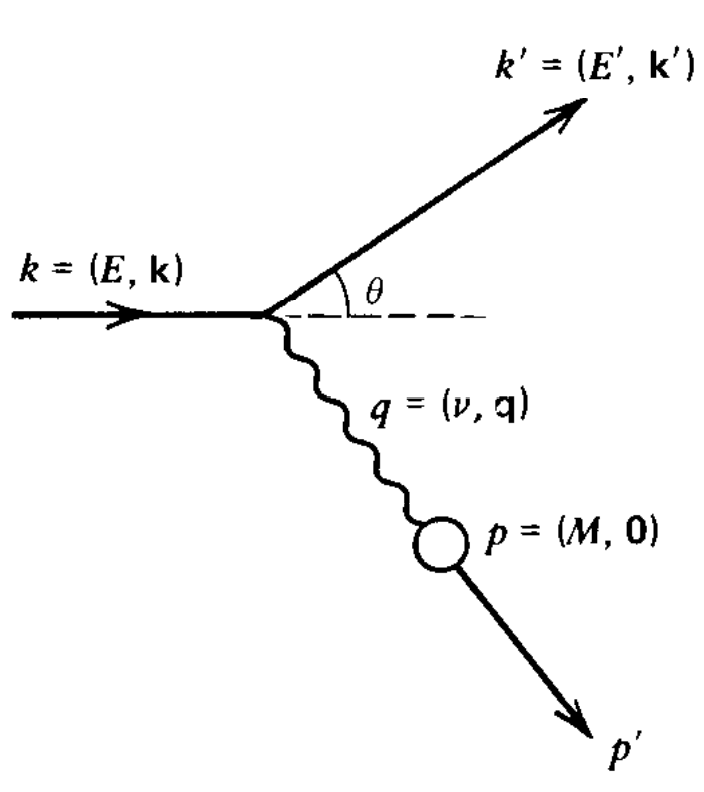
\includegraphics[width=0.4\linewidth]{gallery/background/emu_lab.png}
    \caption{Cartoon depiction of $e^-\mu^-\rightarrow e^-\mu^-$ scattering in the lab frame. Figure from Halzen \& Martin \cite{Halzen_Martin}.}
    \label{f.emu_lab}
\end{figure}
%
In determining particle collisions and cross-sections, our main objective is to calculate the invariant amplitude $\mathcal{M}$, which encodes the physics of the interaction. Since $\mathcal{M}$ is Lorentz-invariant, we can choose a reference frame that is easy to work with. One common choice is the lab frame, in which the muon is initially at rest. We can also assume that the electron mass is negligible, i.e. $m_e\approx 0$, since it is much smaller than all other energy scales in the interaction. Fig. \ref{f.emu_lab} illustrates how this interaction looks in the lab frame. The electron hits a stationary muon, then scatters off at an angle $\theta$ with respect to its initial direction of motion. A photon is exchanged, transferring some four-momentum from the electron to the muon, which then recoils. The four-momenta are
\begin{center}
\begin{equation}
\begin{aligned}
    & k = (E,\mathbf{k}) \\ 
    & k' = (E,\mathbf{k'}) \\
    & q \equiv (\nu, \mathbf{q}) = k-k' \\
    & p = (M,\mathbf{0}) \\ 
    & p' = p+q \ ,
    \label{eqn.k_p_q}
\end{aligned}
\end{equation}
\end{center}
where $M$ is the muon mass. It follows from the relativistic mass-energy-momentum relation, $m^2=E^2-|\mathbf{p}|^2$, that if the electron is approximately massless, $E^2\approx|\mathbf{k}|^2$ and $(E')^2\approx|\mathbf{k'}|^2$. Then $\mathbf{k}\cdot\mathbf{k'}=|\mathbf{k}||\mathbf{k'}|\cos{\theta}\approx EE'\cos{\theta}$.

Let us bring our attention to the exchanged photon. Unlike the electron and muon, which are {\it external} particles, the photon does not appear in the initial nor final state, but is a completely {\it internal} propagator. Its role is to mediate the interaction, carrying four-momentum between the electron and muon. In other words, the amount of four-momentum transferred from the electron to the muon, $q\equiv(\nu, \mathbf{q})=k-k'$, is precisely the four-momentum of the photon. (By conservation of four-momentum, we also have $q=p'-p$.) We can calculate $q^2$ in the lab frame:
\begin{equation}
\begin{aligned}
    q^2 &= (k-k')^2 \\
    &= k^2 + (k')^2 - 2k\cdot k' \\
    &= 2m_e^2 - 2 k\cdot k' \\
    &\approx -2k\cdot k' \ ,
\end{aligned}
\end{equation}
where $k^2=(k')^2=m_e^2\approx0$ by the relativistic mass-energy-momentum relation. Then by definition of the dot product between four-momenta, $k\cdot k'\equiv EE'-\mathbf{k}\cdot\mathbf{k'}$, and
\begin{equation}
\begin{aligned}
    q^2 &= -2(EE'-|\mathbf{k}||\mathbf{k'}|\cos{\theta}) \\
    &\approx -2EE'(1-\cos{\theta}) \ .
\end{aligned}
\end{equation}
% (For more details about manipulating four-momenta, see Appendix \ref{sec.relativity}.)

We find that $q^2$ is in general nonzero,
% Thus, $q^2\neq m_\gamma^2$, seemingly breaking the laws of relativity. Vaguely speaking, the Heisenberg uncertainty principle $\Delta E \Delta t \geq 1 / 2$ provides some leeway, allowing such particles to fluctuate into existence for an extremely brief, unobservable, amount of time. 
meaning $q^2\neq m_\gamma^2$. (Although we performed the calculation in the lab frame, $q^2$ is Lorentz-invariant, so its value is the same in every reference frame.) This photon does not obey the relativistic mass-energy-momentum relationship, and therefore it must be fundamentally unobservable. Such particles are termed {\it virtual}, or {\it off-shell}. In general, all internal propagators are virtual particles. (They are sometimes labeled with a $*$ symbol, like $\gamma^*$ in Fig. \ref{f.emu_emu}.)

In processes like $e^-\mu^-\rightarrow e^-\mu^-$, we use the square of the four-momentum transfer, $q^2$ to quantify the energy of the scattering interaction. Since $q^2<0$, we define the positive variable 
\begin{equation}
    Q^2 \equiv -q^2 \ .
\end{equation} 
In Ch. \ref{sec.bkg_dis_dsigma}-\ref{sec.bkg_dis_partons}, we will apply these kinematics to examine $ep$ scattering.

%-----------------------------
% \subsection{$ep$ scatterings and proton structure}
% \label{sec.bkg_ep}
% %
% In this section, we will discuss the cross sections of $ep$ scattering interactions and how they relate to proton structure....

% %
% \begin{figure}[h!]
%     \centering
%     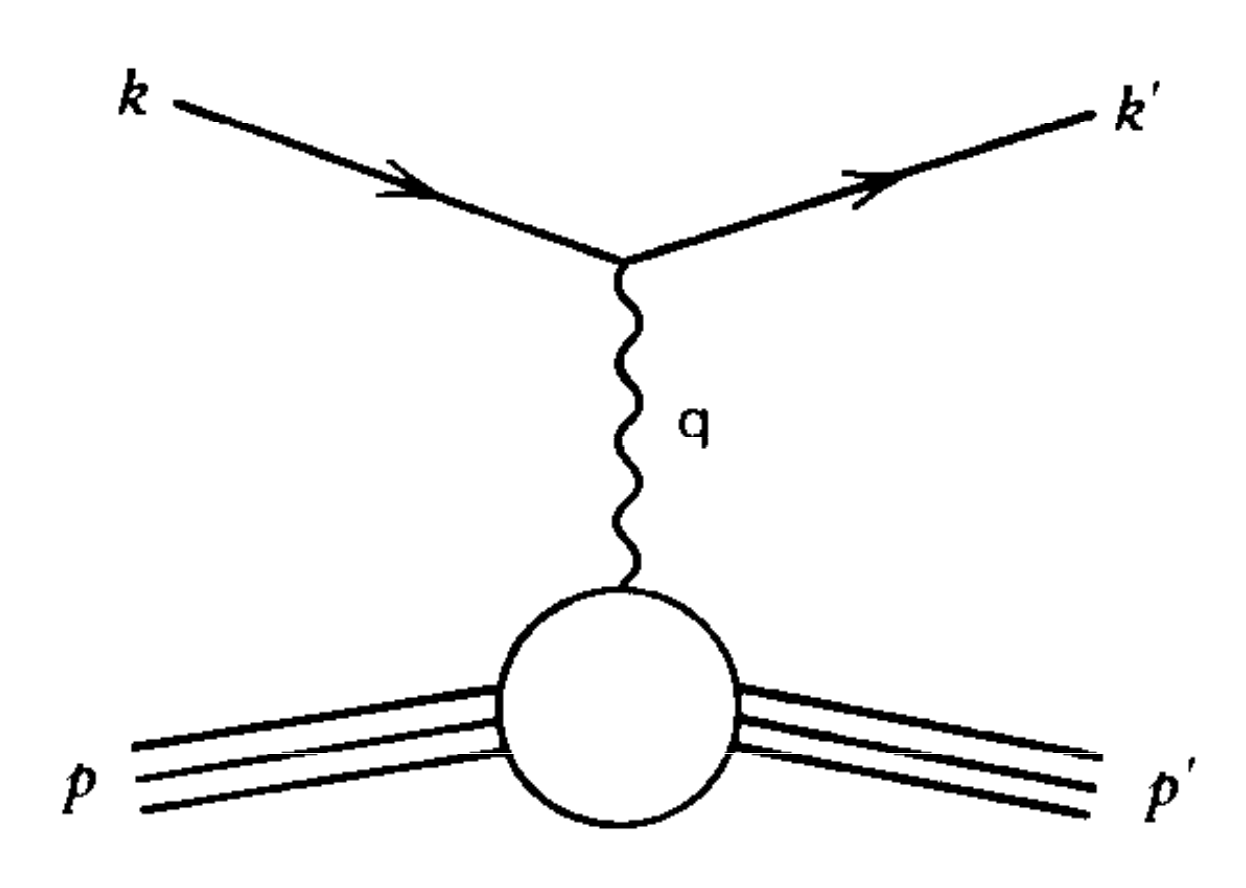
\includegraphics[width=0.5\linewidth]{gallery/background/ep_ep.png}
%     \caption{Leading order Feynman diagram for elastic electron-proton scattering, $e^-(k) + p(p) \rightarrow e^-(k') + p(p')$. Figure from Halzen \& Martin \cite{Halzen_Martin}.}
%     \label{f.ep_ep}
% \end{figure}
% %
% The Feynman diagram for $e^-+p\rightarrow e^-+p$, shown in Fig. \ref{f.ep_ep}, has the same general structure as the diagram for $e^-+\mu^-\rightarrow e^-+\mu^-$ in Fig. \ref{f.emu_emu}. In fact, the top half of the diagrams, which deals with the electron, are identical. However, in the bottom half of Fig. \ref{f.ep_ep}, we now have a proton, which is a complex hadron composed of quarks and gluons. We draw the proton propagator with multiple lines and the proton-photon vertex as a blob, representing the ambiguity about what the particles are inside the proton and how they interact with the photon. In the following discussion, we will parametrize how the proton, being a particle with nontrivial structure, affects the scattering cross section.

% As for the $e\mu$ scattering example in Ch. \ref{sec.bkg_emu}, let us consider the $ep$ scattering in the lab frame, with the proton is initially at rest, and assume that the electron is approximately massless. The $ep$ interaction looks exactly like the illustration in Fig. \ref{f.emu_lab}, with the same four-momenta as those listed in Eq. \eqref{eqn.k_p_q}. 
% % The electron travels toward the proton with initial four-momentum $k=(E,\mathbf{k})$, exchanges a virtual photon with four-momentum $q\equiv(\nu,\mathbf{q})=k-k'$, then scatters off with a new four-momentum $k'=(E',\mathbf{k'})$ such that $\mathbf{k}\cdot \mathbf{k'}=|\mathbf{k}||\mathbf{k'}| \cos{\theta}=EE'\cos{\theta}$. The proton has an initial four-momentum $p=(M,\mathbf{0})$, where $M$ is its mass, and recoils with final four-momentum $p'=p+q$.

% If the proton were a point particle, like the muon, then the differential cross section would be
% \begin{equation}
%     \left(\frac{d\sigma}{d\Omega} \right)_{\rm point} = \left( \frac{\alpha}{2E\sin^2\frac{\theta}{2}} \right)^2 \frac{E'}{E} \left[ \cos^2\frac{\theta}{2}-\frac{q^2}{2M^2}\sin^2\frac{\theta}{2} \right] \ ,
%     \label{eqn.ep_ep_point}
% \end{equation}
% where $d\Omega=r^2\sin{\theta}drd\theta d\phi$ is the solid-angle where the scattered particles are measured, $\theta$ is the polar angle with respect to the particle beam axis (the $z$-axis), and $\alpha$ is the electromagnetic coupling. $k=(E,\mathbf{k})$ is the four-momentum of the incoming electron, $k'=(E',\mathbf{k'})$ is that of the outgoing electron, and $q=(\nu,\mathbf{q})$ is that of virtual photon (see Eq. \eqref{eqn.k_p_q}).

% However, because the proton has some structure, the cross section is given by the more complicated {\it Rosenbluth formula}:
% \begin{equation}
%     \left(\frac{d\sigma}{d\Omega} \right)_{ep\rightarrow ep} = \left( \frac{\alpha}{2E\sin^2\frac{\theta}{2}} \right)^2 \frac{E'}{E} \left[ {\color{purple}\frac{G_E^2(q^2)+\tau G_M^2(q^2)}{1+\tau} }\cos^2\frac{\theta}{2}-{\color{purple}2\tau G_M^2(q^2)}\sin^2\frac{\theta}{2} \right] \ ,
%     \label{eqn.ep_ep_dsigma}
% \end{equation}
% where $M$ is the proton mass, $\tau=-q^2/4M^2$, and $G_E(q^2)$ and $G_M(q^2)$ are two independent functions of $q^2$. The function $G_E$ and $G_M$ essentially modify Eq. \eqref{eqn.ep_ep_point} to account for the effects of proton structure on the scattering interaction. At leading order, $e^-+p\rightarrow e^-+p$ is also an electrodynamic interaction, since it is mediated by a virtual photon. Thus, $G_E$ and $G_M$ are called the electric and magnetic {\it form factors}. They encode information about the electric charge density and magnetic current density of the proton, which we can probe through elastic $ep$ scattering experiments.

%-----------------------------
\subsection{Deep-inelastic scattering: the $ep\rightarrow eX$ cross section}
\label{sec.bkg_dis_dsigma}
In 1969, Richard Feynman proposed the idea that nucleons are composed of point-like {\it partons}, which we now identify as the quarks and gluons of the Standard Model.
In this section and the next, we discuss the characteristics of deep-inelastic scattering (DIS) and how such experiments allow us to probe the partons within the proton. 

% In general, $ep$ collisions can be elastic, with the electron and proton scattering off each other similarly to $e^-\mu^-\rightarrow e^-\mu^-$. They can also be inelastic, in which the proton breaks apart and new particles are produced. The most relevant interaction for this work is deep-inelastic scattering (DIS), $ep\rightarrow eX$ (where $X$ represents any particles).

%
\begin{figure}[h!]
    \centering
    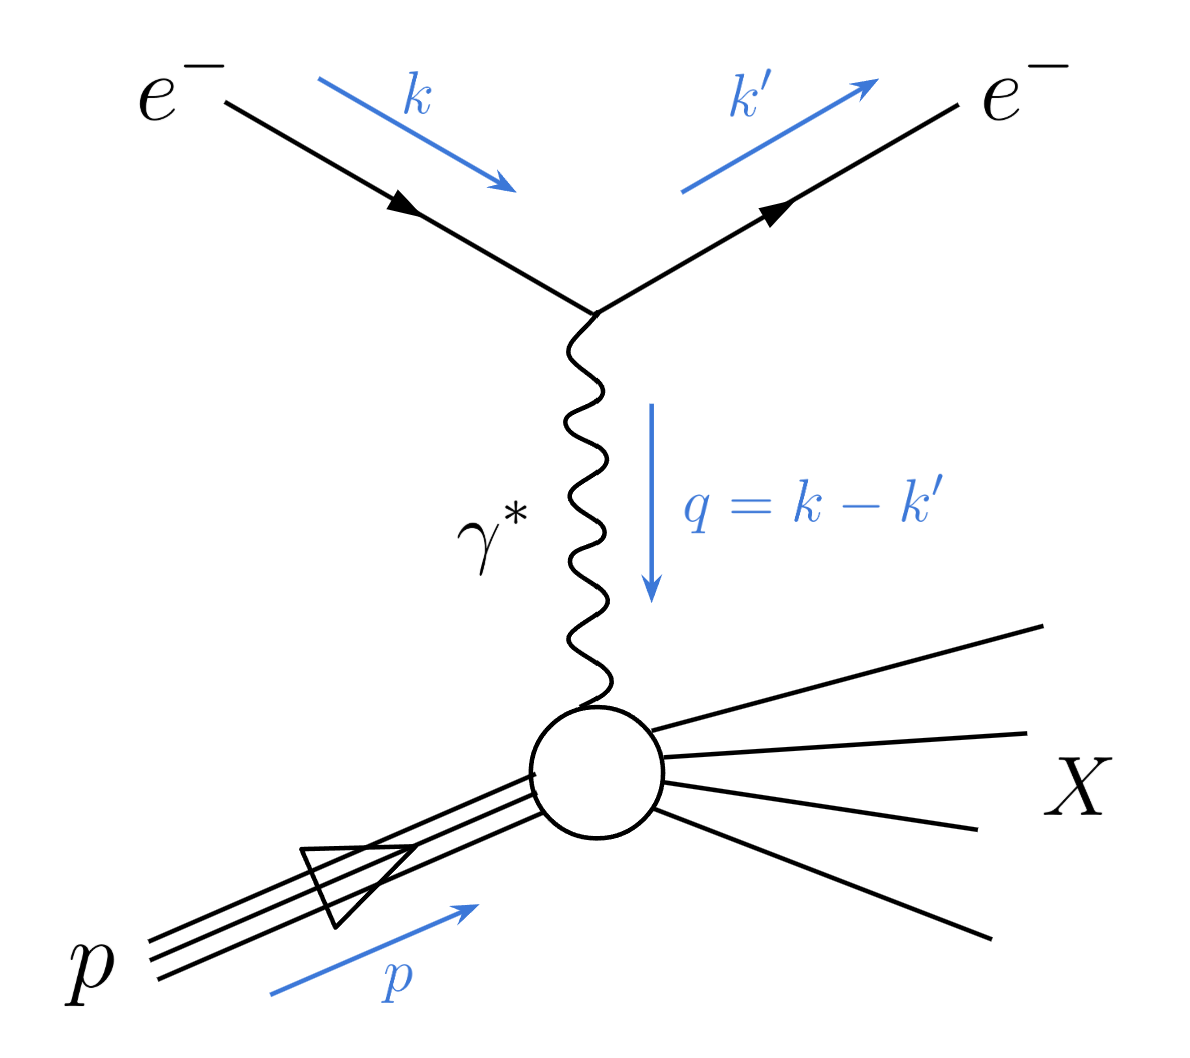
\includegraphics[width=0.4\linewidth]{gallery/background/ep_eX.png}
    \caption{Leading order Feynman diagram for the inelastic scattering $e^-(k) + p(p) \rightarrow e^-(k') + X$. Four-momenta are labeled in blue.}
    \label{f.ep_eX}
\end{figure}
%
The leading order Feynman diagram for DIS, $ep\rightarrow eX$ (where $X$ refers to any particles), is shown in Fig. \ref{f.ep_eX}. The process is similar to that for $e^-\mu^-\rightarrow e^-\mu^-$ in Fig. \ref{f.emu_emu}. In fact, the top half of the diagrams, which deals with the electron, are identical. In the bottom half, we now have an incoming proton, which is subsequently broken up during the interaction, and an array of new particles $X$ is produced.

Unlike the muon, the proton is a complex hadron with internal structure. We draw the proton propagator with multiple lines and its interaction vertex as a blob to represent ambiguity about what exactly the particles are inside the proton and how they interact. In order to examine proton structure, it is not necessary to measure all the particles produced, and we simply denote them collectively as $X$. We refer to such measurements as {\it inclusive}, meaning that we remain agnostic about the final state particles $X$ and, in our calculations, simply sum over all the possible final states. (Measurements can also be semi-inclusive, if we measure one or a few of the particles produced.)

As we did for the $e\mu$ scattering example in Ch. \ref{sec.bkg_emu}, let us consider $ep\rightarrow eX$ in the lab frame, with the proton is initially at rest, and assume that the electron is approximately massless. If the proton were a point particle, the interaction would look exactly like the illustration in Fig. \ref{f.emu_lab}, with the same four-momenta as those listed in Eq. \eqref{eqn.k_p_q}. 
% For the electron,
% \begin{equation}
% \begin{aligned}
%     k &= (E,|\mathbf{k}|) \\
%     k' &= (E'|\mathbf{k'}|) \ ,
% \end{aligned}
% \end{equation}
% with $\mathbf{k}\cdot\mathbf{k'}\approx EE'(1-\cos{\theta})$. For the virtual photon,
% \begin{equation}
%     q=(\nu, \mathbf{q}) = k-k' ,
% \end{equation}
% and for the proton,
% \begin{equation}
% \begin{aligned}
%     p &=(M,\mathbf{0}) \\
%     p' &= p+q \ ,
% \end{aligned}
% \end{equation}
% where $M$ is the proton mass.
The differential cross section would be \cite{Halzen_Martin}
\begin{equation}
    \left(\frac{d\sigma}{d\Omega dE'} \right)_{\rm point} = \left( \frac{\alpha}{2E\sin^2\frac{\theta}{2}} \right)^2 \frac{E'}{E} \left[ \cos^2\frac{\theta}{2}+\frac{Q^2}{2M^2}\sin^2\frac{\theta}{2} \right] \delta\left(\nu - \frac{Q^2}{2M} \right) \ ,
    \label{eqn.ep_point}
\end{equation}
where $d\Omega=r^2\sin{\theta}drd\theta d\phi$ is the solid-angle where the scattered particles are measured, $\theta$ is the polar angle with respect to the particle beam axis (the $z$-axis), and $\alpha$ is the electromagnetic coupling. $k=(E,\mathbf{k})$ is the four-momentum of the incoming electron, $k'=(E',\mathbf{k'})$ is that of the outgoing electron, and $q=(\nu,\mathbf{q})$ is that of the virtual photon, with $Q^2=-q^2$. The delta-function $\delta\left(\nu -{Q^2}/{2M} \right)$ restricts the values of the photon energy to $\nu=Q^2/2M$.

However, because the proton has some structure, the differential cross section involves a bit more complexity \cite{Halzen_Martin}:
\begin{equation}
    \left(\frac{d\sigma}{d\Omega dE'} \right)_{\rm DIS} = \left( \frac{\alpha}{2E\sin^2\frac{\theta}{2}} \right)^2 \frac{E'}{E} \left[ {\color{purple}\frac{F_2(Q^2,\nu)}{\nu}}\cos^2\frac{\theta}{2}-{\color{purple}\frac{2F_1(Q^2,\nu)}{M}}\sin^2\frac{\theta}{2} \right] \ ,
    \label{eqn.ep_eX}
\end{equation}
where $F_1$ and $F_2$ are {\it structure functions} that modify Eq. \eqref{eqn.ep_point} to account for the effects of proton structure on the scattering interaction. In addition, $\nu$ is now independent of $Q^2$, as reflected by the absence of the delta-function term.

%-----------------------------
\subsection{Deep-inelastic scattering: from proton to partons}
\label{sec.bkg_dis_partons}
What do the structure functions $F_1$ and $F_2$ reveal about the proton? In the $ep\rightarrow eX$ Feynman diagram of Fig. \ref{f.ep_eX}, we can think of the virtual photon as our probe into the proton. For very high energy collisions, the energy of the photon is large, so its wavelength is small. Thus, the higher the energy, the smaller the distance scales the experiment can resolve. In the regime of deep-inelastic scattering, the energy is high enough for the photon to probe individual partons. 

In fact, in the {\it Bjorken limit}, in which $Q^2\rightarrow\infty$ and $\nu\rightarrow\infty$ while their ratio remains finite, we can model DIS as elastic scatterings of the electron with a single quark inside the proton. In this regime, $F_1$ and $F_2$ no longer scale separately with $Q^2$ and $\nu$, but only depend on the ratio
\begin{equation}
    x \equiv \frac{Q^2}{2M\nu} \ , \label{eqn.bjorken}
\end{equation}
called {\it Bjorken-$x$}.

% To interpret this Bjorken-$x$ variable, let us consider deep-inelastic scattering $ep$ scattering in the limit where the motion of all particles is along the particle beams. 
% This is known as the infinite-momentum frame, in which the proton has momentum $|\mathbf{p}|\equiv p_z\rightarrow\infty$. In this limit, all partons inside the proton have such large momenta in the $z$-direction, that we can assume their motion to be collinear to the proton and neglect any transverse momentum.
%
\begin{figure}[h!]
    \centering
    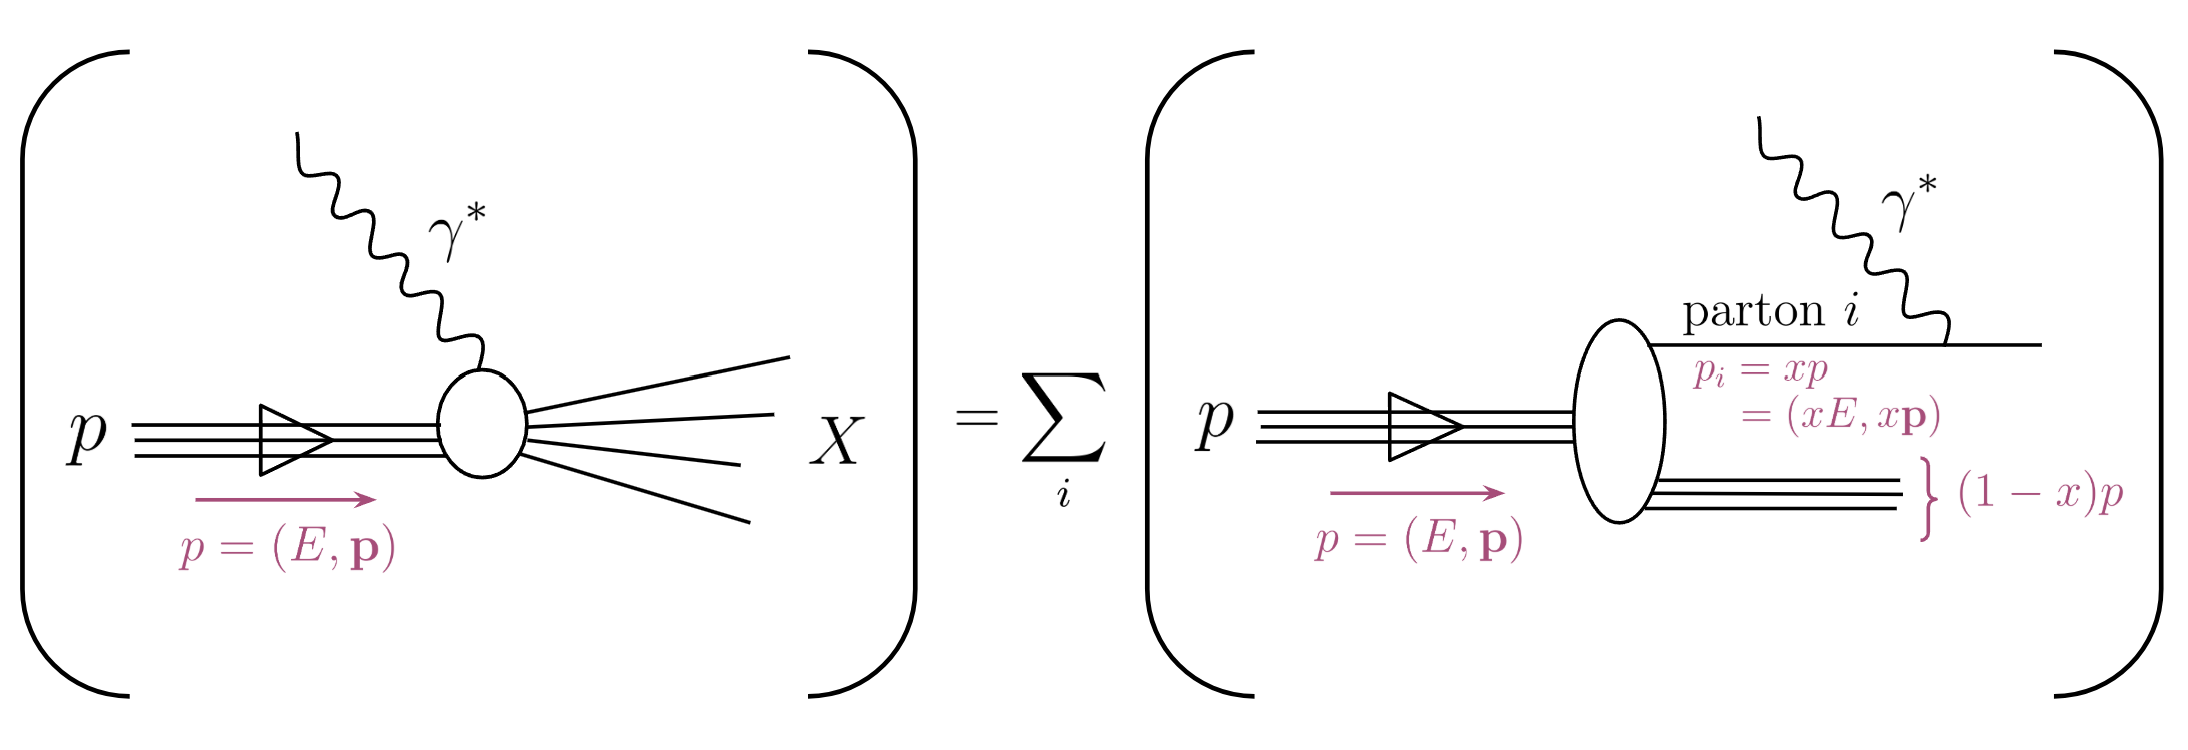
\includegraphics[width=0.95\linewidth]{gallery/background/ep_parton.png}
    \caption{Cartoon depiction of the $\gamma^*p$ interaction in $ep\rightarrow eX$ as the sum of $\gamma^*$-parton interactions in the infinite momentum frame. Four-momenta are labeled in magenta. Figure adapted from Halzen \& Martin \cite{Halzen_Martin}.}
    \label{f.ep_parton}
\end{figure}
%
Figure \ref{f.ep_parton} depicts the $\gamma^*p$ interaction in $ep\rightarrow eX$ (the lower half of Fig. \ref{f.ep_eX}) as the sum of all possible interactions between $\gamma^*$ and a parton $i$ inside the proton. (For simplicity, let us assume all partons are traveling in the same direction as the proton.) For a proton with four-momentum $p=(E,\mathbf{p})$, a given parton $i$ has four-momentum $p_i=xp$. In other words, Bjorken-$x$ is the parton {\it momentum fraction}, the fraction of the proton momentum carried by a given parton. 

The structure functions are given by \cite{Halzen_Martin}
\begin{equation}
    2xF_1(x) = F_2(x) = \sum_i e_i^2xf_i(x) \ ,
    \label{eqn.F1_F2}
\end{equation}
where $e_i$ is the electric charge of parton $i$ in units of the proton charge (e.g. $e=2/3$ for up quarks, $e=-1/3$ for down quarks, and $e=0$ for gluons), and $f_i(x)$ is known as the {\it parton distribution function}. The parton distribution function, defined by
\begin{equation}
\begin{aligned}
    dP_i &= f_i(x) \ dx \\
    1 = \sum_idP_i &= \sum_i \int_0^1 f_i(x) \ dx \ ,
    \label{eqn.pdf}
\end{aligned}
\end{equation}
is the probability density of finding a parton of flavor $i$ with momentum fraction $x$. In other words, $f_i(x)$ describes the momentum-space distribution of partons inside the proton. (Technically, only the quarks contribute to Eq. \eqref{eqn.F1_F2}, since gluons have no electric charge. The gluons contribute to $ep\rightarrow eX$ through higher order terms, such as in the photon-gluon fusion process in Fig. \ref{f.ccbar}.)

Beyond the collinear parton distribution functions (PDFs) described in Eq. \eqref{eqn.pdf}, a variety of more complex observables have been formulated to capture various aspects of quark and gluon dynamics. For example, transverse-momentum dependent (TMD) PDFs account for both the collinear and transverse motion of partons, generalized parton distributions (GPDs) describe the parton distributions in three-dimensional position-space, and polarized versions of these functions describe the distribution of spin among the partons \cite{pdfs}.


% We can check that this parton model makes some sense if we consider the $x\rightarrow 1$ limit (as if the proton were one large parton). If $x=1$ and $e=1$ (the proton charge), then $f(x)=1$ and $\nu=Q^2/2M$ (see Eq. \eqref{eqn.bjorken}), which means 
% \begin{equation}
% \begin{aligned}
%     F_2(x) &= 1 \\
%     2F_1(x) &= \frac{1}{x} = \frac{2M\nu}{Q^2}
% \end{aligned}
% \end{equation}
% This reduces Eq. \eqref{eqn.ep_eX} for the $ep\rightarrow eX$ cross section to Eq. \eqref{eqn.ep_point}, the cross section for a hypothetical point-like proton.

%---------------------------------------------------------
\section{The Electron-Ion Collider (EIC) and the search for Color Glass Condensate (CGC)}
\label{sec.bkg_EIC}

The Electron-Ion Collider (EIC) \cite{EIC} is a new particle collider currently being built at Brookhaven National Lab, designed to image protons and nuclei with unprecedented precision. Through high energy deep-inelastic scattering experiments with electron-proton ($ep$) and electron-ion ($eA$) collisions, the EIC will reveal detailed information about the spatial and momentum distributions of quarks and gluons within protons and nuclei. Measurements of these various parton distributions will bring us closer to understanding the complex dynamics responsible for the generation of mass and spin in nuclear matter.

In particular, the high energies of the EIC will allow us to more effectively study the gluons, which are thought to carry significant contributions to proton mass and spin, yet whose distributions and dynamics are much less understood than those of the quarks. One major phenomena of interest is the existence of a {\it Color Glass Condensate (CGC)}, a theorized state of nuclear matter characterizing the internal structure of protons at very high energies. In this high energy regime---or more precisely, in the regime of small Bjorken-$x$ (defined in Eq. \eqref{eqn.bjorken})---proton structure is dominated by gluons. This is because gluons, being massless particles that can self-interact due to their color charge, will tend to split into more gluons with infinitesimal momentum fraction, forming a highly dense ``condensate" of ``colored" bosons. However, when two gluons meet, they can also recombine into a single gluon, so the gluon density cannot continue to grow unchecked as Bjorken-$x$ approaches 0. Eventually, the rate of gluon splitting ($g\rightarrow gg$) and recombination ($gg\rightarrow g$) will reach an equilibrium, causing the gluon density to {\it saturate}. Additionally, because the gluons are also extremely time-dilated after being accelerated to high energies, they form Classical ``glass"-like fields that evolve very slowly in time. 

Previous experiments at the HERA Collider at DESY in Germany, operational from 1992 to 2007, found signatures consistent with the presence of Color Glass Condensate, but the data did not extend to low enough Bjorken-$x$ to observe true gluon saturation. At the EIC, which is set to begin operations in the 2030s, one overarching goal is to obtain more direct evidence of saturation and study the dynamics of the CGC.

%---------------------------------------------------------
\section{Heavy flavor probes}
\label{sec.bkg_heavy_flavor}

%
\begin{figure}[h!]
    \centering
    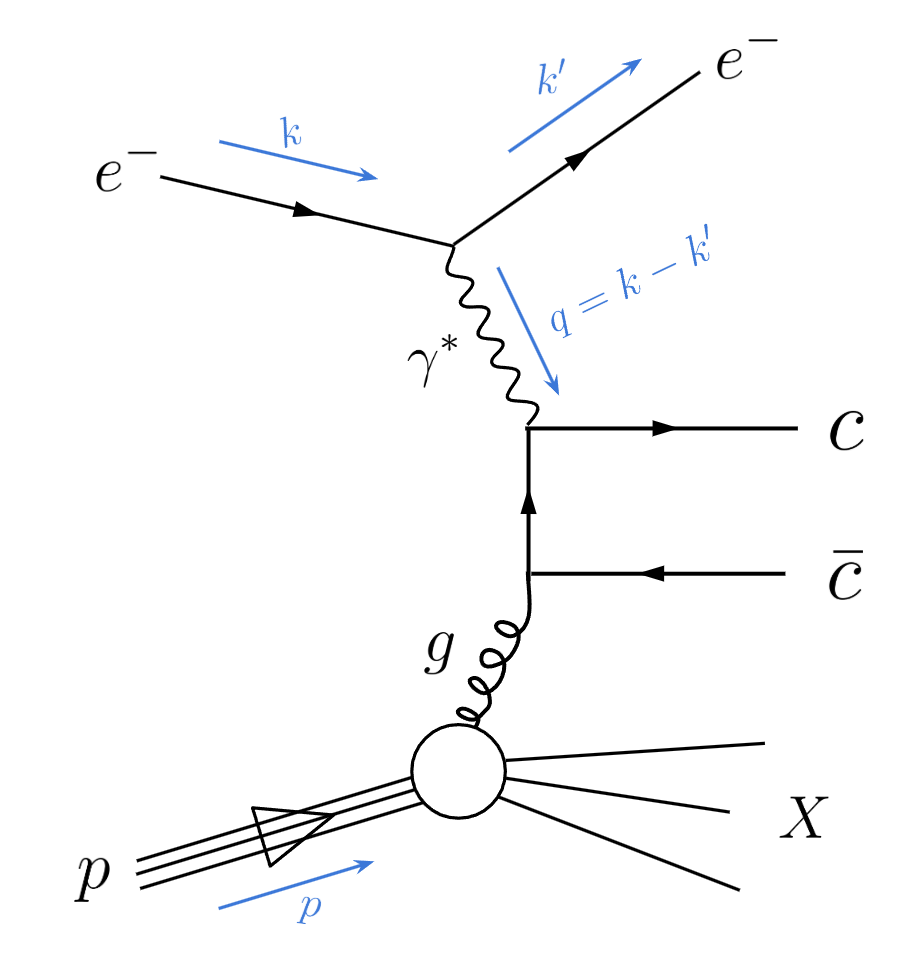
\includegraphics[width=0.4\linewidth]{gallery/background/ccbar.png}
    \caption{Photon-gluon fusion in deep-inelastic scattering, leading to the production of a charm and anti-charm pair.}
    \label{f.ccbar}
\end{figure}
%
During electron-proton and electron-ion collisions at the EIC, interactions involving gluons can lead to the production of {\it heavy flavor} quarks: charm ($c$) and beauty ($b$). The most common of such processes is photon-gluon fusion, depicted in Fig. \ref{f.ccbar}, in which the electron emits a virtual photon, which then interacts with a gluon inside a proton (or neutron) to produce a quark-antiquark pair. Because heavy flavor quarks are so massive, they can only be produced in gluon interactions during the initial high-energy $ep$ collisions. (The masses are around $1~{\rm GeV/c^2}$ for $c$ and $4~{\rm GeV/c^2}$ for $b$, vs. only $1~{\rm GeV/c^2}$ and $5~{\rm GeV/c^2}$ for the most common $u$ and $d$ quarks, respectively.) Thus, heavy flavor quarks carry information about the initial collision conditions, serving as high-sensitivity probes to the gluon distributions and dynamics we wish to study.

After being produced, quarks will immediately hadronize into color-neutral bound states. Consequently, we must study heavy flavor quarks through the hadrons they form, such as the $D^0$-meson, which is the subject of this analysis. In Chapter \ref{ch:d0_top}, we will discuss our method of analyzing these short-lived $D^0$-mesons in $ep$ collisions at the EIC.